\chapter{Introduction} \label{chap:intro} 

Modern applications of machine learning have become ubiquitous, 
to the point where almost all
interactions with so-called ``smart"
technologies involve some
call and response with some form of
learned predictor.
The large scale of these models,
up to billions of parameters in neural networks,
makes possible what would otherwise
be an unconstrained, infeasible learning task
via a highly parameterized model.
These parameterizations have enabled 
human-level performance on learning tasks
previously thought to have been insurmountable
for any potential artificial intelligence system.
The high accuracy and generalization of these large scale models notwithstanding,
a number of parallel questions have arisen and are gaining prominence with respect to 
the performance of these models.
What features are most important for prediction?
Which samples were most important for my training?
Can we understand when a model is certain or uncertain about its output?
Are there layers in my network that have learned a particular subtask?
Questions of robustness, bias, influence, fairness, and importance have become central questions to contemporary machine learning research \citep{doshi2017towards,mehrabi2021survey,amodei2016concrete}.

Traditional statistical learning methods 
have been studied with these questions in mind for many decades, and have found new life in these subfields.
Linear regressors, decision trees, and support vector machines
have all been analyzed under these lenses,
and as the modern machine learning community
has returned to these questions
so has a renewed interest in their methods of analysis.
New research focuses
particularly on the differences
associated with moving from classical under-parametrized models to
modern \textbf{over-parameterized} models: where
the model dimension vastly outnumbers the number
of input samples, and may even be comparable to 
the \textit{entire sample space.}
While nascent, these new methods and analyses
attempt to fill the gap between
statistical and deep models to enable similar measures of sample influence, feature importance, and model understanding. 

% Significant progress in the modern development of machine learning has
% been built upon connections and patterns identified across myriad
% interdisciplinary fields of study.
% Up through the mid 2000's, 
% many of these methods were inspired by and interested in 
% highly focused and constrained problems. 
% With a reasonably sized input domain, could a model of roughly equal size be used to
% predict some output?
% Linear regressors, decision trees, and support vector machines were all answers to these questions, with their own
% varying degrees of scaling and complexity.
% These methods necessitated carefully constructed formulations with specific restrictions to the learnable function class,
% enabling straightforward analysis 
% for provable performance guarantees 
% and easy identification of critical training samples and important input features.

% Contemporary machine learning, however, has a vastly different modus operandi. 
% Driven in large part by the exponential growth of available computation via Moore's Law, \textit{deep learning} has fallen squarely in the realm of \textbf{over-parameterized} models.
% With these overparametrizations and computation capacity, the typical learning questions posed as maximizing accuracy or reducing error have largely been addressed for even large scale problems.
% As such, complementary questions have led to subfields focusing on other performance measures, such as robustness, fairness, interpretability, and explainability.
% Many solutions to these questions end up looking back at answers found for the under- or non-parametrized settings.
% While nascent, these approaches 
% attempt to fill the gap between
% statistical and deep models to enable similar measures of sample influence, feature importance, and model analysis. 
% Most notable amongst these newer approaches is that of (Self)-Attention in Neural Networks \citep{sutskever2014sequence,vaswani2017attention}.
% Other proposals 
% end up looking back at the types of analysis typical of those more classical under-parametrized or nonparametrized methods.

% Not limited to previous developments in learning or computation theory, the arguably most valuable contributions toward the exponential reduction in model error can be attributed to influences and intuitions taken
% from biology, psychology, neuroscience, and even XXX \citep{srivastava, etc}.
% Perhaps one explanation as to why this phenomenon exists may be attributed to the way in which deep learning evolved. 
% The classical learning goal of function approximation lends itself nicely to a system which allows for arbitrary complexity via simple changes (e.g., addition of neural network layers). % Foundational works building on the original neural networks particularly have taken advantage of constraining this space of functions to search over: 
% the most seminal case being those of convolutional filters for imaging data. 
% While ``constraints" of this form have helped tremendously in model performance on modern vision and language machine learning tasks (GANs, Recurrent Networks, Residual Layers, Transformers, etc.), the ability to identify \textit{subsets} of important samples, input features, and model parameters has lagged significantly behind the development of these methods.
% Recently larger interest has been taken by the community to understand and interpret models with this view, only after extremely large and opaque models have become ubiquitous.
%This lag directly explains the more recent interest in developing methods for understanding and interpreting large scale machine learning models.


\paragraph{A full picture.} Consider a dataset $\{X\}_{i=1}^n$ of size $n$ where each data point in the set $X$ is considered drawn from some underlying distribution over the domain $X \sim \cX^d$, with domain dimensionality $d$. A model $f$ is fit using a parametrizations $\theta \in \Theta$, with $\Theta$ the space of possible parametrization with some intrinsic dimension $p$. From an analysis perspective, we might be interested in any one of (a) subsets of input features $\cC \subseteq \cX$ that are important for the downstream task, (b) associating model subsets $\cP \subseteq \Theta$ with specific inputs or groups of inputs, or (c) subsets or subgroups of samples $S \subseteq \{X\}^n$ equally of interest. While all three of these problems are closely related, they require different approaches. 

\begin{mdframed}[style=MyFrame]
\em 
\textbf{This thesis} will focus its main efforts on identifying these important subsets of model, feature, and sample space for feature association, model size reduction, model unlearning, and, fairness. Specifically, taking advantage of both existing statistical and geometric methods, we will develop new methods for localizing subsets, in a range of settings from hypothesis testing on the one hand to deep learning frameworks on the other.
\end{mdframed}

% Features
Feature selection in the case of typical regression or classification
% Typical regression or classification 
takes some form of learning parameters $\theta$ that allow for $\hat{y} = f_\theta(x)$ to be close to the true outcome of interest $y$.
While forms of data $X := (x,y)$ may simply be continuous and real-valued, modern machine learning has greatly expanded formulations of the classical learning problem to include a wide variety of structured learning problems \citep{nowozin2011structured}. 
% Structure learning and identification has taken a few different forms (object detection, segmentation, etc.),
% but has remained somewhat removed from traditional
% statistical settings.
Consider the case when a high-dimensional input is used to predict an output with a highly-parametrized model. 
Once learned, obvious questions arise as discussed above: are there specific low-dimensional spaces in either the input or the model space that are most important or necessary for the global learning problem of interest? Are there specific subspaces associated with particular subproblems of the global problem?
The machine learning literature has come up with a number of ways to identify analogs of these spaces, 
including extensions of sensitivity analysis to deep learning \citep{yeung2010sensitivity,zhang2015sensitivity}, and constructing and identifying nonzero model subsets via particular model choices such as activations \citep{selvaraju2017grad} and regularizers.
In classical settings these are well understood: decision trees naturally provide ease of interpretibility via the information used to choose splits, and both linear and kernel support vector machines have been analyzed to provide for measures of sample importance via distances to the margin as well as feature importance via weights defining the learned hyperplane \citep{Mitchell97}.
Attention and saliency maps have emerged as popular new methods,
given their ease of implementation and interpretation \citep{sutskever2014sequence,vaswani2017attention,selvaraju2017grad}.
By learning dimensions of a given input that are particularly important, either in a hard (binary) or soft (continuous weighting) manner, model builders are better able to understand and interpret what a model has learnt.

The specific ideas of attention notwithstanding, many of these existing methods are far removed from traditional hypothesis testing frameworks.,
While some work has begun in this direction \citep{tansey2018black},
there remains a gap in direct identification of subsets and structures in these spaces that can be defined in statistically rigorous manners.

\paragraph{A specific example.} Consider a traditional machine learning classification task in which we would like to predict whether an individual has a specific disease condition based on a medical resonance image (MRI) scan of their brain. Our input feature $x$ may consist of a 3D-array of values lying in $\RR^{x\times y\times z}$ measuring some intensity of the imaging modality at each voxel, indexed by a tuple $(i,j,k)$.
Our outcome variable $y$ may simply be a binary label of whether the input scan has been labeled by a radiologist as one demonstrating typical disease characteristics.
Using an off the shelf 3D convolutional neural network with adjustments to match our input size, we can very quickly set up and train a system to predict disease presence with a high degree of accuracy.

While attention can be directly applied to the network in order to identify ``hotspots" in the input space relating to the learned classification task, 
given the high-dimensional nature of the input
and the relatively small sample size 
associated with medical imaging data, 
it is very likely that an area of interest identified
may be an intricacy of the training samples used rather than truly a region of disease signal.
Class activation maps (CAMs) may be unclear, and can often associate with image artifacts unrelated to the scientific task \citep{adebayo2018sanity}.
Methods of generalization may help to increase confidence in identified regions, but statistical guarantees often remain out of reach.

Furthermore, most recent problems associated with medical data have moved past simple difference detection: trends over time, and the ability to predict {\em future} disease development has by far become the setting of most interest.
Given an image of a healthy individual, is it possible to predict what their scan, or their future disease diagnosis, may be up to 10, 20, or more years in the future?
If a number of scans have been collected over some timeframe, can the \textit{trajectory} of the individuals' development be extrapolated to estimate progression?
As traditional models extended for temporal analysis grow in both size and complexity,
a number of subproblems explicitly related to model and input subspaces arise. Here we aim to address two such problems: \textbf{statistically rigorous identification of temporally evolving subsets}, and \textbf{characterizations of deep models that enable efficient training of recurrent models with large scale time-varying data}.

With the rapid growth of AI and machine learning applications has come valid concerns regarding both guarantees of privacy.
Recent technology legislation has made the importance clear in all aspects of data use,
and particular projects and groups have demonstrated that machine learning is not independent of
this need \citep{Exposing}.
A new issue raised within this intersection is the ``right to be forgotten".
If a model has been trained with a particular users' data, 
they should have some recourse or right
to both remove their data from the training set,
and also know that the model has not learned from their data.
On the surface, this poses a significant problem for model builders
and organizations that spend large amounts
of time and resources in 
training deep learning models.
As we will see, 
\textbf{identification of model parameter subsets}
that are particularly important
for a particular sample's influence
in a model enables \textit{efficient machine unlearning}.

% para - connections to geometric deep learning, graph NNs, etc.


A sample's particular influence on model parameters aside, the identification of influential samples or subsets of samples more generally is of independent interest. 
Traditionally a rigorous area of study under classical statistics, outlier detection and accounting have become a subfocus for many within the machine learning community as well \citep{golatkar2020eternal,golatkar2020forgetting,huang2020feature,ren2019likelihood}.
While subgroups of input samples may be outliers, it is more often the case that they represent known heterogeneity within the data. 
These differences are typically marked using 
group information known a priori, and 
most learning tasks aim to learn tasks
in a \textit{subgroup-independent} manner.
Optimization and regularization methods with this focus come under the umbrella of model fairness, and instead of identifying and boosting independences within the model or data, we aim to minimize them.
However, many existing methods do not scale well as the number of subgroups grows, as is often the case when intersections of protected classes must be considered. In the sequel we identify and construct a particular solution for \textbf{groupwise fairness that enables efficient in the loop fairness regularization}.

\begin{mdframed}[style=MyFrame]
\textbf{ Thesis Goal: }
\em Identify, construct, and evaluate methods for subset identification in machine learning input, feature, and model spaces, taking advantage of inherent geometric and statistical structures that naturally arise in application domains. 
Application focus is put on scientific domains in healthcare and social equity.
\end{mdframed}

\section{Thesis Scope and Contributions}

In this thesis we explore the intersections of classical statistical and geometric constructions with modern machine learning methods. 
Figure~\ref{fig:scope} shows the overall scope projected along three axes: feature, parameter, and sample spaces.
Below we briefly introduce the main problems studied in this thesis.
\begin{figure}[!ht]
    \centering
    % \includegraphics[width=0.99\linewidth]{scope.pdf}
    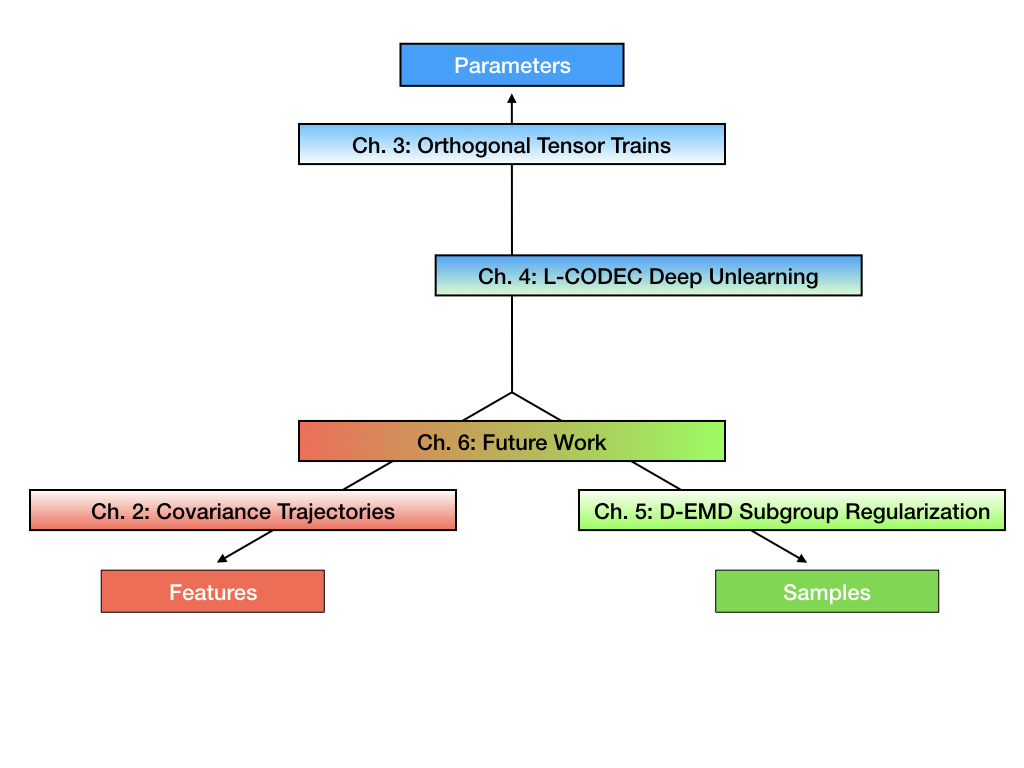
\includegraphics[width=0.95\linewidth]{_introduction/thesis_scope.png}
    \caption{Thesis scope, projected over three representative axes.}
    \label{fig:scope}
\end{figure}

\subsection{Second-Order Modeling and Group Difference Analysis over Time}

Recent results in coupled or temporal graphical models offer schemes for estimating the relationship structure 
between features when the data come from
related (but distinct) longitudinal sources. A novel application of these ideas is for analyzing group-level differences, i.e., in identifying if {\em trends} of estimated objects (e.g., 
covariance or precision matrices) are different across disparate conditions (e.g., gender or disease). Often, poor effect sizes make detecting the \textit{differential} signal 
over the {\em full} set of features difficult: for example, 
dependencies between only a {\em subset of features} may manifest differently across groups.
We first suggest
a parametric model 
for estimating trends in the space of $\SPD$ matrices as a function of one or more covariates.
We will then generalize scan statistics to graph structures, 
to search over distinct subsets of features (graph partitions) whose temporal dependency structure may show statistically 
significant group-wise differences.
We will theoretically analyze the Family Wise Error Rate (FWER) and bounds on Type 1 and Type 2 error. 
On a cohort of individuals with risk factors for Alzheimer's disease (but otherwise cognitively healthy), 
we aim to 
find scientifically interesting 
group differences where the default analysis, 
i.e., models estimated on the {\em full graph}, do not survive reasonable 
significance thresholds. 
Preliminary work on this was published in \citep{covtraj}.


\subsection{Efficient Tensor Representations for Feasible Temporal Deep Learning}

Modern deep networks have proven to be very effective for analyzing real world images.
However, their application in medical imaging is still in its early stages,
primarily due to the large dimension of three-dimensional images, requiring enormous convolutional or fully connected layers --
if we treat an image (and not image patches) as a sample. 
These issues only compound when the focus moves towards longitudinal analysis
through recurrent structures, and when a point estimate of model parameters is insufficient 
in scientific applications where a reliability measure is necessary.
Using insights from differential geometry, 
we will adapt 
the tensor train decomposition to construct networks
with significantly fewer parameters,
allowing us to train powerful recurrent networks on whole brain image volumes. 
We propose 
the \textit{orthogonal tensor train},
and demonstrate its ability to express a standard network layer both theoretically and empirically.
We will 
demonstrate its ability to 
effectively reconstruct whole brain volumes
with faster convergence and stronger confidence intervals
compared to the standard tensor train decomposition. 
We provide code and show experiments on the ADNI dataset
using image sequences to regress on a cognition related outcome.
Preliminary work on this was published in \citep{ott}.

\subsection{Practical Unlearning via Large-Scale Conditional Independence Testing}

%With AI systems extensively using personal %data for model training, 
Recent legislation has
led to interest in {\em machine unlearning}, i.e., removing specific training samples from a {\em predictive} model as if they never existed in the training dataset. 
Unlearning may also be required due to  corrupted/adversarial data or simply a user's updated privacy requirement.
For models which require no training ($k$-NN), 
simply deleting the closest original sample can be effective. 
%However, it is not clear how such approaches can be used to unlearn 
%models that contain rich information learned from the original data.
But this idea is inapplicable to models which learn richer 
representations.
%from data. 
%Recently, optimization-based unlearning estimators have been proposed, but 5their 
Recent ideas leveraging optimization-based updates
scale poorly with the model dimension $d$,  
due to 
inverting the Hessian of the loss function. %with an overall cost of $O(d^3)$ 
%is prohibitive.
We propose
a variant of a new conditional independence coefficient, 
L-CODEC, to identify a subset of the model parameters with the most semantic overlap on an individual sample level. 
Our approach completely avoids the need to invert a (possibly) huge matrix. 
By utilizing a Markov blanket selection, 
we premise
that L-CODEC is also suitable for deep unlearning,
as well as other applications in vision.
Compared to alternatives, L-CODEC makes approximate unlearning possible 
in settings that would otherwise be infeasible, 
including vision models used for face recognition, 
person re-identification 
and NLP models that may require unlearning samples identified for exclusion.
Preliminary work on this will appear in \citep{lcodec}.


\subsection{Reducing Subgroup Fairness via High Dimensional Earth Mover's Distances}

Optimal transport has recently emerged as a useful tool for machine learning through its connections with geometry, statistical machine learning, and through practical algorithms. Existing methods that leverage optimal transport often  regularize using  a Wasserstein metric or by computing barycenters, for example. %which are effective when distributions are continuous and known, or when measures of interest are discrete.
% Our formulation allows for a discretization of continuous measures that drop in directly to classical  formulations of the Earth Mover's Distance. 
We will leverage optimal transport, except that we take advantage of a recently-introduced algorithm that computes a generalized earth mover's distance.
Not only is this algorithm computationally cheaper to compute compared to existing barycentric measures, but our method has the additional  advantage that gradients used for backpropagation can be directly read off of the forward pass computation, which leads to substantially faster model training.
We will provide technical details about this new regularization term and its properties, 
and 
experimental demonstrations of improved training speed over existing Wasserstein-style methods.

\subsection{Applying Conditional Independence Testing for better Understanding of Preclinical Alzheimer's Disease}

The final chapter of this thesis applies some of the tools developed above in analyzing preclinical Alzheimer's disease patients. 
In these studies, 
we aim to identify conditionally independent features and subjects that are particularly important to the prediction and estimation of
key disease outcomes,
as a function of a number 
of demographic, neuropsychological,
genetic,
and imaging data collected as 
part of an ongoing consortium 
to understand the progression
of Alzheimer's disease in younger, 
asymptomatic populations.
In what follows we present
exploratory analysis
on a small, easily 
digestible subset of the available data,
that lays the foundation for
further analysis.

% This work is the most forward looking, and aims to be a stepping stone toward a rigorous 

\subsection{Outline}
In Chapters 2 through 5, we describe four perspectives to address subset identification.
Chapter 2 explores and focuses on the identification of feature subsets varying over time.
In Chapter 3 we describe a method of constraining the parameter space in a particular manner
that enables more efficient large scale neural networks.
Next, Chapter 4 provides a solution to the machine unlearning problem,
enabled through a particular conditional independence parameter selection scheme, vastly reducing network update costs.
Chapter 5 ends with a unique solution to subgroup fairness, 
where we take advantage of an efficient solution to
the $d$-dimensional earth mover's problem
to regularize large models when the number of subgroups can be large.
Chapter 6 describes future work, focused on applying a particular solution from Chapter 4 to understanding relationships among
disease indicators and biomarkers associated with developing Alzheimer's Disease.